\documentclass[a4paper,titlepage,onecolumn]{report}

% title of the dissertation
\def\distitle{Working Title}
\usepackage{mathtools}
\usepackage{t1enc}
\usepackage[T1]{fontenc}
\usepackage{ulem}
\usepackage{import}
\usepackage{amsmath}
\usepackage{amssymb}
\usepackage{paralist}
\usepackage{booktabs}
\usepackage[version=3]{mhchem}
\usepackage{wrapfig}
\usepackage{pifont}
\usepackage{mathrsfs}
\usepackage{xcolor}
\usepackage{color}
\usepackage{enumitem}
\usepackage{datetime}
\usepackage{fullpage}
\usepackage{hyperref}
\usepackage{attachfile}
\usepackage{textpos}
\usepackage{rotating}
\usepackage{ifthen}
\usepackage[parfill]{parskip}
\usepackage{minted}


\hypersetup{
 colorlinks=true,
 citecolor=black,
 linkcolor=black,
 pdftitle={\distitle}
}

% New definition of square root:
% it renames \sqrt as \oldsqrt
% This definition puts a little vertical guy at the end so it's more
% obvious where the square root actually ends.
\let\oldsqrt\sqrt
% it defines the new \sqrt in terms of the old one
\def\sqrt{\mathpalette\DHLhksqrt}
\def\DHLhksqrt#1#2{%
\setbox0=\hbox{$#1\oldsqrt{#2\,}$}\dimen0=\ht0
\advance\dimen0-0.2\ht0
\setbox2=\hbox{\vrule height\ht0 depth -\dimen0}%
{\box0\lower0.4pt\box2}}

% integrals with infinity bounds
\newcommand{\intinfty}{\int_{-\infty}^{\infty}}

% consistent formatting of object labels
\newcommand{\Figure}[1]{Figure \ref{#1}}
\newcommand{\Equation}[1]{Equation \ref{#1}}
\newcommand{\Table}[1]{Table \ref{#1}}
\newcommand{\Section}[1]{Section \ref{#1}}
\newcommand{\Chapter}[1]{Chapter \ref{#1}}
\newcommand{\Part}[1]{Part \ref{#1}}
\newcommand{\Appendix}[1]{Appendix \ref{#1}}

% I want all of the document numbering to always show the full path, fuck
% with this later
%\renewcommand\thesection{\Roman{part}.\Alph{chapter}.\arabic{section}}
%\renewcommand\thesubsection{\arabic{section}.\arabic{subsection}}
%\renewcommand\thesubsubsection{\arabic{subsection}.\arabic{subsubsection}}

%\renewcommand\thefigure{S\arabic{figure}}
%\renewcommand\thesection{\Roman{part}.\arabic{chapter}.\arabic{section}}
%\renewcommand\thetable{S\arabic{table}}

% names have a particular formatting
\newcommand{\name}[1]{\textsc{#1}}

% missing mathematical operators
\DeclareMathOperator{\sinc}{sinc}
\DeclareMathOperator{\sech}{sech}
\DeclareMathOperator{\sgn}{sgn}
\DeclareMathOperator{\erf}{erf}
\DeclareMathOperator{\inverf}{inverf}
\DeclareMathOperator{\arcsinh}{arcsinh}
\DeclareMathOperator{\arccosh}{arccosh}
\DeclareMathOperator{\arctanh}{arctanh}
%\DeclareMathOperator{\Re}{Re}
%\DeclareMathOperator{\Im}{Im}

% use roman type for natural base e and sqrt(-1)
\newcommand{\me}{{\mathrm{e}}}
\newcommand{\mi}{{\mathrm{i}}}

% roman type for the derivative, plus a space
\newcommand{\md}{\,\mathrm{d}}

% fourier transform and the reverse
\newcommand{\ff}[1]{{\mathscr{F}^{+}\bigl(#1\bigr)}}
\newcommand{\fr}[1]{{\mathscr{F}^{-}\bigl(#1\bigr)}}

% hilbert transform and the reverse
\newcommand{\hf}[1]{{\mathscr{H}^{+}\bigl(#1\bigr)}}
\newcommand{\hr}[1]{{\mathscr{H}^{-}\bigl(#1\bigr)}}

% QCM related frequency and bandwidth shifts
\newcommand{\df}{\Delta\!f}
\newcommand{\dg}{\Delta\Gamma}
\newcommand{\xil}{\xi_\mathrm{L}}
\newcommand{\kl}{k_\mathrm{L}}
\newcommand{\ml}{m_\mathrm{L}}
\newcommand{\kq}{k_\mathrm{q}}
\newcommand{\mq}{m_\mathrm{q}}
\newcommand{\omegaq}{\omega_\mathrm{q}}

\newcommand{\thetasp}{\theta_\mathrm{sp}}

% custom lengths for figures

% width for side by side figures
\newlength{\twoupwidth}
\setlength{\twoupwidth}{7.5cm}

% width and height for default single figure
\newlength{\oneupwidth}
\setlength{\oneupwidth}{0.90\textwidth}
\newlength{\oneupheight}
\setlength{\oneupheight}{0.55623059\textwidth}

\usepackage{pgfplots}
\usepackage{pgfplotstable}
\pgfplotsset{compat=newest}
\usepgfplotslibrary{units}
\usepgfplotslibrary{external}
\pgfplotsset{filter discard warning=false}

\usepackage[siunitx]{circuitikz}
\usepackage{tikz}
\usetikzlibrary{calc}
\usetikzlibrary{patterns,decorations.pathmorphing,decorations.markings,positioning}
\usetikzlibrary{pgfplots.units} 
\usetikzlibrary{pgfplots.external} 
\usetikzlibrary{pgfplots.groupplots}
%\tikzexternalize[prefix=external/]% externalize

% my pretty colors
% \import{colors/}{colors}

% siunitx
\usepackage{siunitx}
\DeclareSIUnit\molar{\mole\per\cubic\deci\metre}
\DeclareSIUnit\Molar{\name{M}}

\sisetup{ 
% load-configurations=abbreviations
% round-mode = places,
}%

% set PDF attributes
\pdfpageattr {/Group << /S /Transparency /I true /CS /DeviceRGB>>} 

% prettify chapter/section format
\usepackage{titlesec}
\newcommand{\hsp}{\hspace{20pt}}
\titleformat{\chapter}[hang]{\Huge\bfseries}{\thechapter\hsp\textcolor{gray}{|}\hsp}{0pt}{\Huge\bfseries}

\begin{document}

%%%%% TITLE PAGE %%%%%
\begin{titlepage}
\begin{center}
\hfill\\[4cm]
{ \Huge {\bfseries {\distitle}} \par}
\vspace{3.0cm}
\begin{tabular}{lr}

\includegraphics[height=2cm,keepaspectratio]{images/Logo_MPL_englisch_kompakt_cmyk_110915}
\hspace{1.0cm}
%

\includegraphics[height=2cm,keepaspectratio]{images/Logo_IMPRS_4c_042012}
\end{tabular}
\vspace{3cm}
\\
{\huge Aaron Webster}\\
\vspace{1cm}
{\large A DISSERTATION}\\
\vspace{0.5cm}
Presented to the Max Planck Institute for the Science of Light\\
and the University of Erlangen-N\"urnberg\\
in partial fulfillment of the requirements\\
for the degree of\\
Doctor of Philosophy\\
\vspace{0.5cm}
\today
\end{center}
%\tikzexternaldisable
\tikz[overlay,remember picture] {
 \node at ($(current page.west)+(1,0)$) [rotate=90]
 {\large\textcolor{gray}{\input{commithash} \pdfdate}};
}
%\tikzexternalenable
\end{titlepage}

%%%%% DECLARATION OF ORIGINALITY %%%%%
\chapter*{Declaration of Originality}
I affirm that the work presented in this dissertation is, to the best of my
knowledge, original and my own, except as acknowledged in the
text. \\
\hfill\\[1cm]
Signed\hspace{0.25cm}\makebox[5cm]{\hrulefill}\hspace{0.25cm}(Aaron Webster)
\hfill\\[1cm]
Date\hspace{0.51cm}\makebox[5cm]{\hrulefill}\hspace{0.25cm}
\vspace{2cm}

%%%%% ADVISOR, CO-ADVISOR %%%%%
\section*{Evaluation Committee}
\subsection*{First Advisor}
Dr. Rer. Nat. Frank Vollmer\\
Laboratory of Biophotonics and Biosensing\\
Max Planck Institute for the Science of Light\\
G\"unther-Scharowsky-Str.1 / Bau 24\\
91058 Erlangen
\subsection*{Second Advisor}
Prof. Dr. Ulf Peschel\\
Institute of Optics, Information and Photonics\\
University Erlangen-N\"urnberg\\
G\"unther-Scharowsky-Str.1 / Bau 24\\
91058 Erlangen

\newpage
%%%% ACKNOWLEDGEMENTS %%%%
\chapter*{Acknowledgements}
I would like to extend my sincerest gratitude to the following individuals
who contributed to this work: \name{Jiapeng~Huang}, for his enthusiasm
and hard work in carrying out many tedious but necessary experiments,
\name{Yuqiang~Wu} for establishing the DNA origami and related protocols,
\name{Matthew~Foreman} for carrying out insightful theoretical modeling
regarding SPP multiple scattering, \name{Frank~Vollmer} for his optimism
in seeing this work to a successful completion, \name{Stephen~Gregory}
and \name{R\@.P.\@~Schumann} whose pioneering experiments are the basis
for my own, and \name{Yuki~Sato} for his patience and progressive
scientific ideas regarding his centrifugal force quartz crystal
microbalance.  Most significantly, I would like to recognize
\name{Norbert~Lindlein}, without whom this dissertation would not be
possible.

%%%%% TABLE OF CONTENTS &&&&&
\pagenumbering{roman}
\tableofcontents

%%%%% ABSTRACT %%%%%
\begin{abstract}
 Abstract is written last.
\end{abstract}
% the first part is in roman numbering, switch now to arabic
\pagenumbering{arabic}




\section{Geometry}


\begin{figure}
 \caption{Geometry for computing specklegrams.}
\end{figure}

% limits for 2D
\begin{align}
 f(x)=\sqrt{x^2+z^2}-\sqrt{\left(x+\delta\right)^2+z^2}
\end{align}
\begin{align}
 \lim_{x \to 0} f(x)
 &= \lim_{x \to 0} \sqrt{x^2+z^2}-\sqrt{\left(x+\delta\right)^2+z^2} \\
 &= z-\sqrt{\delta^2+z^2}
\end{align}

For $\delta \ll z$, the limit is $0$.

\begin{align}
 \lim_{x \to \infty}f(x)
 &=\lim_{x \to \infty}\sqrt{x^2+z^2}-\sqrt{(x+\delta)^2+z^2} \\
 &= \lim_{x \to \infty}\frac{\left(\sqrt{x^2+z^2}-\sqrt{\left(x+\delta\right)^2+z^2}\right)\left(\sqrt{x^2+z^2}+\sqrt{\left(x+\delta\right)^2+z^2}\right)}
 {\sqrt{x^2+z^2}+\sqrt{\left(x+\delta\right)^2+z^2}}\\
 &= \lim_{x \to \infty}\frac{-2\delta}
 {\sqrt{x^2+z^2}+\sqrt{\left(x+\delta\right)^2+z^2}}\\
 &=\lim_{x \to \infty}\frac{x}{|x|}\frac{-\frac{\delta^2}{x}-2\delta}
 {\sqrt{1+\frac{z^2}{x^2}}+\sqrt{1+\frac{z^2}{x^2}+\frac{2\delta}{x}+\frac{\delta^2}{x^2}}}\\
 &=\frac{-2\delta}{\sqrt{1}+\sqrt{1}}\\
 &=-\delta
\end{align}


% correlations radially tell you about the z height things


\begin{figure}[ht]
\centering
\begin{tikzpicture}
\begin{axis}[
xlabel=$\theta$,
ylabel=correlation coefficent,
thick,
small,
width=\oneupwidth,
height=0.75\oneupheight,
minor tick num=2,
legend pos = north east,
legend style = { cells = {anchor=west} },
restrict x to domain=0:0.1,
%restrict y to domain=0:0.5,
trim axis left,
]
\addplot[color=colora] file {speckle/radcor/3_xcov_nscat_10.dat};
\addplot[color=colorb] file {speckle/radcor/4_xcov_nscat_20.dat};
\addplot[color=colorc] file {speckle/radcor/5_xcov_nscat_50.dat};
\addplot[color=colord] file {speckle/radcor/6_xcov_nscat_100.dat};
\legend{10,20,50,100}
\end{axis}
\end{tikzpicture}
\end{figure}

\begin{figure}[ht]
\centering
\begin{tikzpicture}
\begin{axis}[
xlabel=$\theta$,
ylabel=correlation coefficent,
thick,
small,
width=\oneupwidth,
height=0.75\oneupheight,
minor tick num=2,
legend pos = north east,
legend style = { cells = {anchor=west} },
restrict x to domain=0:0.1,
%restrict y to domain=0:0.5,
trim axis left,
]
\addplot[color=colora] file {speckle/radcor/2_xcov_theta_40.dat};
\addplot[color=colorb] file {speckle/radcor/3_xcov_theta_50.dat};
\addplot[color=colorc] file {speckle/radcor/4_xcov_theta_60.dat};
\addplot[color=colord] file {speckle/radcor/5_xcov_theta_70.dat};
\legend{\SI{40}{\degree},\SI{50}{\degree},\SI{60}{\degree},\SI{70}{\degree}}
\end{axis}
\end{tikzpicture}
\end{figure}

\begin{figure}[ht]
\centering
\begin{tikzpicture}
\begin{axis}[
xlabel=$\theta$,
ylabel=correlation coefficent,
thick,
small,
width=\oneupwidth,
height=0.75\oneupheight,
minor tick num=2,
legend pos = north east,
legend style = { cells = {anchor=west} },
restrict x to domain=0:0.1,
%restrict y to domain=0:0.5,
trim axis left,
]
\addplot[color=colora] file {speckle/radcor/1_xcov_scanxy_1.0000000000000000818e-05.dat};
\addplot[color=colorb] file {speckle/radcor/2_xcov_scanxy_2.0000000000000001636e-05.dat};
\addplot[color=colorc] file {speckle/radcor/3_xcov_scanxy_3.000000000000000076e-05.dat};
\addplot[color=colord] file {speckle/radcor/4_xcov_scanxy_4.0000000000000003272e-05.dat};
\legend{\SI{10}{\micro\meter},\SI{20}{\micro\meter},\SI{30}{\micro\meter},\SI{40}{\micro\meter}}
\end{axis}
\end{tikzpicture}
\end{figure}

%\section{Calculating the Sensor Distance}
The way the experiment is constructed makes it difficult to accurately
measure the distance between the imaging sensor and the focal spot.
However, with knowledge of the angle in which the sensor is tilted, this
distance can be extracted \textit{a posteriori} from measuring the shape
of the light falling on the sensor.
\begin{figure}
\centering
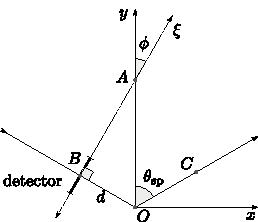
\includegraphics[keepaspectratio,scale=1.25]{figures/hyperbolageoa.pdf}
\caption{Geometry for determining the sensor distance $d$.}
\label{fig:propgeo}
\end{figure}

Consider the experimental geometry.  Light from scattered SPPs eminates as
a cone and is imaged by a planar sensor.  This is by definition a conic
section, with the SPP light cone as the cone and the sensor as the cutting
plane.  Following, the shape of the light on the sensor will be either a
circle, an ellipse, a parabola, or a hyperbola.  In the experimental setup
we can easily set things up such that sensor is fixed
orthogonal to the SPP cone.  The geometrical situation is depicted in
\Figure{fig:propgeo}.  SPPs eminate into the far field from point $O$ at
$\thetasp$.  The detector, which has a finite length, is at $B$ and is
orthogonal to $\overline{OB}$ at an angle $\phi=\pi/2-\thetasp$ with respect to
the normal vector from the prism surface $\overline{OA}$.  Because
$\phi<\thetasp$ and $\thetasp>\pi/2$, lines $\overline{BA}$ and $\overline{OC}$ never
intersect. The resulting shape is a hyperbola.  We wish to determine, given
the parameters of the hyperbolic section, the distance between the focal
spot and the sensor $d$.  

We denote the coordinates of the sensor as $(\xi,y)$.  Here we have the
following relationships
\begin{align}
x &= \xi \cos \thetasp\\
r &= \left(d \sec \thetasp + \xi \sin \thetasp\right) \tan\thetasp
\end{align}
and
\begin{equation}
x^2+y^2=r^2
\end{equation}
Note $d \sec\thetasp$ is the length of $\overline{OA}$.  These two sets of
equations can be combined to obtain
\begin{equation}
\xi^2 \left(\cos ^2\thetasp-\sin ^2\thetasp \tan
^2\thetasp\right)+2 \xi d \tan ^3\thetasp+y^2=d^2 \tan
^2\thetasp \sec ^2\thetasp
\end{equation}
Which, after a bit of algebra, can be solved for $\xi$, taking
the positive root
\begin{equation}
\xi(y) = \frac{4 \sqrt{2} \sqrt{-2 y^2 \cos 2 \thetasp  \cos ^6\thetasp +d^2
\cos ^6\thetasp -d^2 \cos 2 \thetasp  \cos^6\thetasp}-2 d \sin 2 \thetasp
+d \sin 4 \thetasp }{2 \left(2 \cos 2 \thetasp +\cos 4 \thetasp +1\right)}
\label{eqn:conic02}
\end{equation}

To find the offset, we solve the above minimum and find $\xi(y=0) = 4 d
\sec\thetasp$, subtracting this from \Equation{eqn:conic02}.  The remaining
equation is then solved for $d$.
\begin{align}
d =& \Biggl(-4 \sqrt{2} \Bigl(\delta^2 \sin ^2\thetasp \cos
^4\thetasp+\delta^2 \sin ^2\thetasp \cos \thetasp \cos ^4\thetasp-4 y^2 \\
   & \sin ^2\thetasp \cos ^5\thetasp-6 y^2 \sin ^2\thetasp
     \cos ^4\thetasp-16 y^2 \sin ^2\thetasp \cos \thetasp\\
  & \cos ^4\thetasp+4 y^2 \sin ^2\thetasp \cos \thetasp
    \cos ^4\thetasp-8 y^2 \sin ^2\thetasp \cos \thetasp \cos
    ^4\thetasp\Bigr)^{1/2}\\
&-2 \delta\sin \thetasp-4 \delta \sin 3 \thetasp+\delta  \sin \thetasp-4 \delta \sin \thetasp\Biggr)\\
&\cdot\Bigl(4 \left(2 \cos \thetasp+3 \cos \thetasp-3 \cos \thetasp+\cos 5 \thetasp-2 \cos \thetasp-1\right)\Bigr)^{-1}
\end{align}


$\delta$ is the distance the cone goes up at the coordinate $y$.  All you
need is the pixel dimensions and this equation will get you what you want.

%\chapter*{Foreword}
%
%\label{part:plasmon}
%\chapter{Preface}
%\label{ch:preface}
%\section{Synopsis}
%\label{sec:synopsis}
%This dissertation is all about what happens when surface plasmon polaritons
%interfere and scatter in a prism coupled setup.  The easiest way of
%understanding this is though a simplified dipiction of the experimental
%setup, shown in \Figure{fig:kretschmanngeo}.  
%
%\begin{figure}[hb]
%\centering
%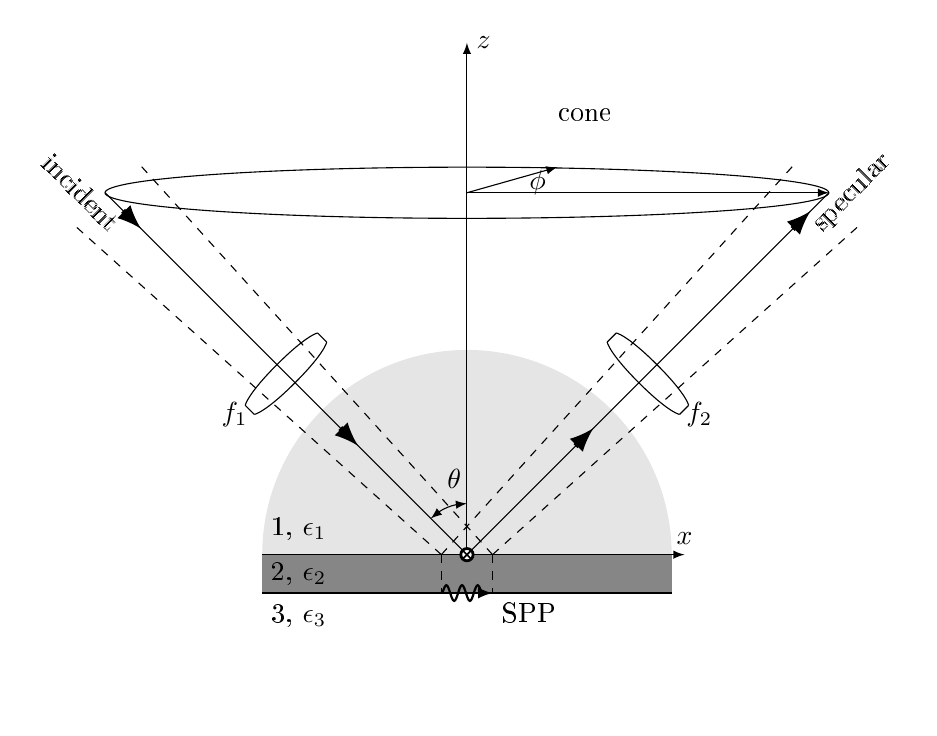
\begin{tikzpicture}[
    scale=0.65,
    >=latex,
    media/.style={font={}},
    wave/.style={
        decorate,decoration={snake,post length=1.0mm,amplitude=1mm,
        segment length=2.0mm},thick},
    interface/.style={
        % The border decoration is a path replacing decorator. 
        % For the interface style we want to draw the original path.
        % The postaction option is therefore used to ensure that the
        % border decoration is drawn *after* the original path.
        postaction={draw,decorate,decoration={border,angle=-45,
                    amplitude=0.3cm,segment length=2mm}}},
    ]

    \def\thetasp{45}
    \def\spread{10}
    \def\wx{1}
    \def\conedist{10}

    % glass
    \fill[gray!20] (4,0) arc (0:180:4);

    % air
    \fill[gray!0] (-4,-3) rectangle (4,0);

    % metal 
    \fill[gray!95] (-4,-0.75) rectangle (4,0);

    % Interface
    \draw[black,line width=.5pt](-4,0)--(4,0);
    \draw[black,line width=.5pt](-4,-0.75)--(4,-0.75);

    % Vertical dashed line
    %\draw[dashed,gray](0,-3)--(0,3);
    % Coordinates system
    \draw[<->] (4.25,0) node[above]{$x$}-|(0,10) node[right]{$z$};
    \draw[->] (0,{cos(\thetasp)*\conedist}) -- ({sin(\thetasp)*\conedist}, {cos(\thetasp)*\conedist});
    \draw[->] (0,{cos(\thetasp)*\conedist}) --
    ({0.25*cos(\thetasp)*\conedist}, {0.5+sin(\thetasp)*\conedist})
    node[shift={(-0.25,-0.20)}] {$\phi$} ;

    \node[shift={(1.5,{sin(\thetasp)*\conedist-1.5})}] {cone};

    % cone
    \draw (0,{cos(\thetasp)*\conedist}) ellipse ({sin(\thetasp)*\conedist} and 0.5);

    % Incidence
    %\draw[->,wave]
    %     (135:3.2cm)--(135:2.5cm)node[right]{$E_0$};
    \draw[dashed](0:{\wx*-0.5})--({90+\thetasp+\spread*0.5}:10);
    \draw[](0:0)--({90+\thetasp}:10) node[rotate={270+\thetasp}, shift={({0.30*cos(270-\thetasp)},{0.30*sin(270-\thetasp})}] {incident};
    \draw[<->] (0,1) arc (90:{90+\thetasp}:1) node[shift={(0.3,0.5)}] {$\theta$};
    \draw[->,line width=2pt]({90+\thetasp}:9.5)--({90+\thetasp}:9.0);
    \draw[->,line width=2pt]({90+\thetasp}:3.5)--({90+\thetasp}:3.0);
    \draw[dashed](0:{\wx*0.5})--({90+\thetasp-\spread*0.5}:10);
    %\draw[->](0,0.75)arc(90:135:.75cm);

    % Reflection
    %\draw[->,wave]
    %     (45:2.5cm)--(45:3.2cm)node[right]{$E_r$};
    \draw[dashed](0:{\wx*-0.5})--({90-\thetasp+\spread*0.5}:10);
    \draw[](0:0)--({90-\thetasp}:10) node[rotate={90-\thetasp},
    shift={({0.30*cos(270+\thetasp)},{0.30*sin(270+\thetasp})}] {specular};
    \draw[<-,line width=2pt]({90-\thetasp}:9.5)--({90-\thetasp}:9.0);
    \draw[<-,line width=2pt]({90-\thetasp}:3.5)--({90-\thetasp}:3.0);
    \draw[dashed](0:{\wx*0.5})--({90-\thetasp-\spread*0.5}:10);
    \draw[dashed]({\wx*0.5},0)--({\wx*0.5},-0.75);
    \draw[dashed]({-\wx*0.5},0)--({-\wx*0.5},-0.75);
    \draw[->,wave,color=black]
     ({-\wx*0.5},-0.75)--({\wx*0.5},-0.75) node[right,shift={(0,-0.25)}]{SPP};


    % first lens
    \def\lenswidth{2}
    \def\lensheight{0.25}
    \def\lensbow{0.125}
    \def\lensshift{({-5*sin(\thetasp)},{5*cos(\thetasp)})}
    \def\lensrotate{\thetasp}
    \draw[shift={\lensshift}, rotate={\lensrotate}]({-\lenswidth/2},{-\lensheight/2})--({-\lenswidth/2},{\lensheight/2});
    \draw[shift={\lensshift}, rotate={\lensrotate}]({\lenswidth/2},{-\lensheight/2})--({\lenswidth/2},{\lensheight/2});
    
    \draw[shift={\lensshift}, rotate={\lensrotate}] plot [smooth, tension=1.5] coordinates {
    ({\lenswidth/2},{-\lensheight/2}) 
    (0,{-\lensheight/2-\lensbow})
    ({-\lenswidth/2},{-\lensheight/2})
    } node[shift={(-0.25,0)}] {$f_1$};

    \draw[shift={\lensshift},rotate={\lensrotate}] plot [smooth, tension=1.5] coordinates {
    ({-\lenswidth/2},{\lensheight/2})
    (0,{\lensheight/2+\lensbow})
    ({\lenswidth/2},{\lensheight/2}) };
    
    % second lens
    \def\lensshift{({5*sin(\thetasp)},{5*cos(\thetasp)})}
    \def\lensrotate{-\thetasp}
    \draw[shift={\lensshift}, rotate={\lensrotate}]({-\lenswidth/2},{-\lensheight/2})--({-\lenswidth/2},{\lensheight/2});
    \draw[shift={\lensshift}, rotate={\lensrotate}]({\lenswidth/2},{-\lensheight/2})--({\lenswidth/2},{\lensheight/2});
    
    \draw[shift={\lensshift}, rotate={\lensrotate}] plot [smooth, tension=1.5] coordinates {
    ({-\lenswidth/2},{-\lensheight/2})
    (0,{-\lensheight/2-\lensbow})
    ({\lenswidth/2},{-\lensheight/2}) 
    } node[shift={(0.25,0)}] {$f_2$};

    \draw[shift={\lensshift},rotate={\lensrotate}] plot [smooth, tension=1.5] coordinates {
    ({-\lenswidth/2},{\lensheight/2})
    (0,{\lensheight/2+\lensbow})
    ({\lenswidth/2},{\lensheight/2}) };


   % Media names
    \path[media] (-4,.5)  node[anchor=west] {1, $\epsilon_1$}
                 (-4,-.375) node[anchor=west] {2, $\epsilon_2$}
                 (-4,-1.2) node[anchor=west] {3, $\epsilon_3$};

    % $x$ axis
    \filldraw[fill=white,line width=1pt](0,0)circle(.12cm);
    \draw[line width=.6pt] (0,0)
                          +(-135:.12cm) -- +(45:.12cm)
                          +(-45:.12cm) -- +(135:.12cm);
    % To-paths are really useful for drawing curved lines. The above
    % to path is equal to:
    %
    % \draw[-latex,thick](3.2,0.5)node[right]{$\mathsf{S_{1,2}}$}
    %      ..controls +(180:.2cm) and +(up:0.25cm) .. (3,0);
    % Internally the to path is translated to a similar bezier curve,
    % but the to path syntax hides the complexity from the user. 

    % SPP
    %\draw[->,wave,color=black]
    %     (-2,-1.75)--(2,-1.75) node[right]{SPP};

\end{tikzpicture}

%\vspace{-1cm}
%\caption{Simplified experimental setup: surface plasmon excitation using
%the three layer Kretschmann configuration. } 
%\label{fig:kretschmanngeo} 
%\end{figure}
%Light is incident from the left and focussed by lens $f_1$ on to the
%hypotenuse of a hemispherical prism $\epsilon_1$ coated with a thin layer
%of metal, $\epsilon_2$.  The refractive index of
%the sample, $\epsilon_3$, is opposite.  $f_2$ acts to image light exiting
%the system, if required.
%
%The evanescent wave present on the $\epsilon_1$-$\epsilon_2$ boundary with
%a wavenumber $k_x = k_0\sqrt{\epsilon_1}\sin \thetasp$ has an angle such
%that it excites surface plasmon polaritions (SPPs); oscillations of free
%charge strongly coupled to the photons of the incident beam.  The majority
%of light is directed into the specular direction.  Here, re-radiated SPPs
%at $\thetasp$ are antiphase with the excitation beam.  The result is
%interference: a dark band or notch in the reflected field.  The angular
%location of the notch turns out to be extrordinarily sensitive to
%$\epsilon_3$ -- this is the common way to view surface plasmon resonance in
%a biosensing context.  
%
%SPPs will propagate on the $\epsilon_2$-$\epsilon_3$ layer until
%they either decay as heat or scatter into the far field.  During this
%propagation it is possible that surface roughness will elastically modify
%its $k$-vector in the $k_x$-$k_y$ plane.  When this happens, scattered SPPs
%will re-radiate into a thin annular cone at (nearly) the same angle as the
%dark band in the specular direction.
%
%The conically scattered light is of prime importance for us, because within
%this light is found a wealth of information directly related to the SPP
%scattering.  In particular, the cone contains speckle: a seemingly random
%interference pattern resulting from many components with different phases.
%
%\section{What is New Here}
%In many large works it is sometimes difficult to discern what is actually
%new from rehashings of things others have done.  Here I intended to clarify
%this situation.  To this accord, the following is a list of explicitly new
%results which I present:
%
%\begin{description}
%\item[{Interference of Scattered SPPs}]
%For SPPs excited in the Kretschmann configuration with a focussed beam
%whose propagation distance is larger than focal spot, a particular one-sided
%interference pattern, is observed in the specular direction.  This was
%thought to be an interference effect between the specularly reflected beam
%and a re-radiated plasmon component, but we have discovered a further
%insight in intrepreting it as a simple consequence of causality.
%\item[{Bulk Refractive Index Sensitivity}] 
%Using Fourier analysis, we have studied the sensitivity of SPR in an intensity
%interrogation configuration as a function of propagation distance.  This
%provides a useful measure of the sensitivity of the one-sided interference
%pattern found in the specular and conically directed beams.
%\item[{Refractive Index Sensing With Conical Speckle}]
%If the surface is rough, the conically directed light contains speckle.  We
%have analyzed the speckle patterns as a function of changes in bulk
%refractive index.
%\item[{SPP Nanoparticle Scattering}]
%Using the speckle in the cone, we observe the changes in intensity and
%correlation functions associated with the addition or motion of a single
%nanoparticle.
%After writing, update the list with all the new stuff.
%\end{description}
%
%\section{Organization}
%How all this is organized.  Should probably be written last.
%
%
%\chapter{Foundations}
%\label{ch:foundations}
%\section{Historical Perspective}
%The theoretical groundwork for the existence of surface plasmon polaritons
%(SPPs) was first introduced by \name{Richie} in his seminal 1957 paper
%\textit{Plasma Losses by Fast Electrons in Thin Films}
%\cite{ritchie1957plasma}.  Like any scientific work, Richie's was
%incremental and has its roots in earlier theoretical proposals by
%\name{Pines} and
%\name{Bohm}~\cite{bohm1951collective}~\cite{pines1952collective}.
%Ultimately this research functioned to explain the phenomena of sharp and
%spectrally narrow energy losses observed in diffraction gratings by
%\name{Wood} in 1902, known as ``Wood's anomaly''.
%
%Optical excitation of surface plasmons was made accessible through
%pioneering work in the late 1960's by
%\name{Kretschmann}~\cite{kretschmann1968},
%\name{Raether}~\cite{raether1965springer} and
%\name{Otto}~\cite{otto1968excitation}.  These experiments used the
%principle of attenuated total reflection (ATR) to excite surface plasmons
%evanescently, using a prism to match their resonance condition.  A great
%deal of understanding on the topic of surface plasmons took place in the
%subsequent decade, including an improved theoretical understanding based on
%Fresnel relations \cite{chen1976excitation} and descriptions of of
%conically scattered light in the presence of surface
%roughness~\cite{simon1976directional}.  A concise overview of this research
%can be found in~\cite{raether1997surface}.
%
%The introduction of SPR as a biosensing platform began in the early 1980's
%with work by \name{Liedberg}, \name{Nylander} and
%\name{Lundstrom}~\cite{liedberg1983surface} who described the
%extraordinary sensitivity of the surface plasmon resonance condition to
%perturbations in the refractive index of the medium on one side of the
%metal film.  The subsequent commercialization of SPR biosensors has largely
%been influenced by these authors and Pharmacia Biosensor AB (now
%Biacore)~\cite{liedberg1995biosensing}.
%
%The commercial success of biosensors based on surface plasmon resonance
%brought about a knowledge gap between the biosensing community and their
%more theoretical predecessors from whom the field owes its genesis; the
%scope of SPR biosensing experiments is disproportionately narrower than the
%breadth of phenomena discovered since Richie.  As an example particular to
%this dissertation, in 2005 and 2007, two
%papers~\cite{andaloro2005optical}~\cite{simon2007observation} based on
%theoretical work by \name{Chuang}~\cite{chuang1986lateral} and
%\name{Chen} \cite{chen1976excitation} reported a curious interference
%pattern occurring in the specularly reflected light for certain (among
%them, Kretschmann-Raether type) systems illuminated with focused Gaussian
%beams.  This was also independently reported a year later in
%\cite{schumann2008near}.  Interestingly, observation of this interference
%required nothing more than the addition of a lens pair to a fairly
%ubiquitous optical setup, but it somehow escaped attention during earlier
%research.  
%
%The thrust of this work is primarily inspired by experiments done at the
%University of Oregon in the labratory of \name{Stephen Gregory}, summarized
%in a 2009 thesis \textit{Surface Plasmon Random Scattering and Related
%Phenomena} \cite{schumann2009surface} by \name{R\@.P.\@~Schumann}.  Here
%the authors describe plasmon experiments with scanning apertureless
%near-field probes in a Kretschmann-Raether type configuration.  This probe
%(a sharp tungsten tip) is able to elastically scatter SPPs in a way
%analogous to surface roughness, but in this case its location and
%interaction of a single scatterer can be precisely controlled.  We will
%show that similar experiments can be carried out in the context of
%biosensing, using metallic nanoparticles as scatterers.
%
%The final important historical development we cross is that of correlations
%in elastic multiple scattering through disordered media.  Most notable is
%the seminal paper by \name{Feng}, \name{Lee}, \name{Stone}, and
%\name{Douglas}~\cite{feng1988correlations}.  Here it was established that
%the seemingly random fluctuations in the output channel through a
%disordered system are not random at all, but contain correlations which
%track the behavior of the input channel.  In the optical regime these
%fluctuations are known as speckle, whose statistal properties have been
%explored in depth by
%\name{Goodman}~\cite{goodman2007speckle}~\cite{goodman1975statistical}.
%The important implications speckle correlations were perhaps best
%summarized by \name{Berkovits} and
%\name{Feng}~\cite{berkovits1994correlations}.  These works established that
%the multiple scattering regime is extraordinary sensitive to both the
%position~\cite{berkovits1990theory} and
%motion~\cite{berkovits1991sensitivity} of even a single scatterer.  This
%problem has important implications in many diverse fields of study:
%diffusive wave spectroscopy~\cite{pine1988diffusing}, tracking and
%identification of targets with radio waves (the ``cruise missile
%problem''~\cite{atkins1991neural}), fluctuations in signal power in
%cellular telephone networks (Rice fading~\cite{abdi2001estimation}), and
%very recently in detecting stress fractures in aggregates such as
%concrete~\cite{larose2010locating}.  
%
%%Our historical perspective ends here.  Scattering of surface plasmons
%%affords one a unique system with which to study these effects.  By changing
%%the amount of surface roughness, 
%
%\section{Surface Plasmon Polaritons}
%A photon is a quantized oscillation of an electromagnetic field.  When this
%field is in proximity to an interface such as the surface of a metal,
%oscillations of free charge can be induced.  If the field is evanescent in
%both directions orthogonal to the surface, the oscillations become
%localized and are known as surface plasmons (SPs).  Furthermore, if
%conditions exist such that the in-plane momentum and phase of the incident
%photon and the surface plasmon match, the coupling produces a hybrid
%excitation known as surface plasmon polariton (SPP).  An SPP is trapped on
%this interface and propagates until it decays; either re-radiating as a
%photon or being absorbed into the metal as heat.
%
%
%\subsection{Wave Equation}
%Most of the relevant behavior of SPP propagation can be derived from the
%electromagnetic wave equation derived from Maxwell's equations.
%\begin{align}
%\left(\nabla^2-\mu\epsilon\frac{\partial^2}{\partial t^2}\right)\mathbf{E}&=0
%\label{eqn:ewe}
%\end{align}
%This is the electromagnetic wave equation in terms of the electric field.
%Choosing to solve this equation by separation of variables the following
%plane wave solutions can be obtained
%\begin{align}
% \mathbf{E} ( \mathbf{r}, t ) &= \mathbf{E}_0\, \me^{\mi (\mathbf{k} \cdot \mathbf{r} - \omega t )}
%\label{eqn:planewaves}
%\end{align}
%where $k=\omega/c=\omega\sqrt{\epsilon\mu}$.  In this notation,
%$\mathbf{k}$ is the material specific vectorial wavenumber, $\mathbf{r}$ is the
%spatial position, $\omega$ is angular frequency, and $t$ is
%the dimension of time.
%The initial value is chosen with the vectorial constant $\mathbf{E}_0$.
%The magnetic field follows the same form
%\begin{align}
% \mathbf{H} ( \mathbf{r}, t ) &= \mathbf{H}_0\, \me^{\mi (\mathbf{k}
% \cdot \mathbf{r} - \omega t )}
%\end{align} 
%but it is orthogonal $\mathbf{E}$ by
%\begin{align}
%\mathbf{E} \times \mathbf{H} = 0
%\end{align}
%and the two are mutually orthogonal with the direction of propagation
%$\mathbf{k}$.
%
%\subsection{Dispersion Relation}
%With plane wave solutions in hand, boundary conditions consistent with a
%dielectric-metal interface can be imposed.
%At a planar interface, it is convenient to restrict the problem to two
%dimensions; in this case the $x$-$z$ plane as shown schematically in
%\Figure{fig:kretschmanngeosimplified}.  Since $\mathbf{k}=(k_x,0,k_z)$,
%$\mathbf{r}\cdot\mathbf{k}=k_x x + k_z z$ and $\mathbf{E}_0 = (E_x, 0,
%E_z)$, the electric field can be written 
%\begin{align}
%\mathbf{E} ( \mathbf{r}, t ) &= \mathbf{E}_0\, \me^{\mi (\mathbf{k}
%\cdot \mathbf{r} - \omega t )}\\
%\mathbf{E}(x,z,t)&=\begin{pmatrix}
%E_x\\ 0\\ E_z
%\end{pmatrix}
%\, \me^{\mi(k_{x,i}x+k_{z,i}z-\omega t)}
%\label{eqn:planewavexz}
%\end{align}
%The magnetic field propagates in the same direction with the
%same $\mathbf{k}$-vector components, but the direction
%$\mathbf{H}$ must be orthogonal to $\mathbf{E}$ by
%\Equation{eqn:faradayslaw}
%\begin{align}
%\mathbf{H} ( \mathbf{r}, t ) &= \mathbf{H}_0\, \me^{\mi (\mathbf{k}
%\cdot \mathbf{r} - \omega t )}\\
%\mathbf{H}(x,z,t)&=\begin{pmatrix}
%0\\ H_y\\ 0
%\end{pmatrix}
%\, \me^{\mi(k_{x,i}x+k_{z,i}z-\omega t)}
%\end{align}
%At the interface there are two values for the (complex) permittivity,
%$\epsilon_1$ in the dielectric and $\epsilon_2$ in the metal.  Consequently
%there are two sets of plane wave solutions
%\begin{align}
%\left.\begin{aligned}
%\mathbf{H}_1(x,z,t) &=
%\begin{pmatrix}
%0\\
%H_{y,1}\\
%0
%\end{pmatrix} \me^{\mi(k_{x,1}x+k_{z,1}z-\omega t)}\\
%\mathbf{E}_1(x,z,t) &=
%\begin{pmatrix}
%E_{x,1}\\
%0\\
%E_{z,1}\\
%\end{pmatrix} \me^{\mi(k_{x,1}x+k_{z,1}z-\omega t)}
%\end{aligned}
%\right\}& \quad \text{dielectric}, \epsilon_1\label{eqn:planewavedielectric}\\
%\left.\begin{aligned}
%\mathbf{H}_2(x,z,t) &=
%\begin{pmatrix}
%0\\
%H_{y,2}\\
%0
%\end{pmatrix}
%\me^{\mi(k_{x,2}x+k_{z,2}z-\omega t)}\\
%\mathbf{E}_2(x,z,t) &=
%\begin{pmatrix}
%E_{x,2}\\
%0\\
%E_{z,2}\\
%\end{pmatrix}
%\me^{\mi(k_{x,2}x+k_{z,2}z-\omega t)}
%\end{aligned} 
%\right\}&\quad \text{metal}, \epsilon_2
%\label{eqn:planewavemetal}
%\end{align}
%where the subscript designates which material the wave equation refers to.
%(e.g. $\mathbf{E}_1$ is the electric field in the dielectric, $\mathbf{H}_2$
%the magnetic field in the metal, etc.)
%Continuity of \Equation{eqn:planewavedielectric} and
%\ref{eqn:planewavemetal} at this interface requires that
%\begin{align}
%E_{x,2}&=E_{x,1}\\
%H_{y,2}&=H_{y,1}\\
%\epsilon_2 E_{z,2}&=\epsilon_1 E_{z,1}
%\end{align}
%Applying Ampere's law (\Equation{eqn:ampereslaw}) to the field on the
%each boundary gives
%\begin{align}
%\nabla \times \mathbf{H}_i &= \epsilon_i \frac{\partial \mathbf{E}_i}{\partial t}\\
%\begin{pmatrix}
%\frac{\partial H_{z,i}}{\partial y} - \frac{\partial H_{y,i}}{\partial z}\\
%\frac{\partial H_{x,i}}{\partial y} - \frac{\partial H_{z,i}}{\partial z}\\
%\frac{\partial H_{y,i}}{\partial y} - \frac{\partial H_{x,i}}{\partial z}
%\end{pmatrix}
%&= \begin{pmatrix}
%-\mi k_{z,i} H_{y,i}\\
%0\\
%\mi k_{x,i} H_{y,i}
%\end{pmatrix}
%\\
%&= \begin{pmatrix}
%-\mi \omega \epsilon_i E_{x,i}\\
%0\\
%-\mi \omega \epsilon_i E_{z,i}
%\end{pmatrix}
%\label{eqn:vectordisp}
%\end{align}
%where $\mathbf{E}_i$, $\mathbf{H}_i$, $i=1,2$ represent the field in either the
%dielectric or the metal.  The vector components of
%\Equation{eqn:vectordisp} are therefore related 
%\begin{align}
%-\mi k_{z,i} H_{y,i} &= -\mi \omega \epsilon_i E_{x,i}\\
%k_{z,1} H_{y,1} &= \omega \epsilon_1 E_{x,1}\\
%k_{z,2} H_{y,2} &= \omega \epsilon_2 E_{x,2}
%\label{eqn:spderivsteptwo}
%\end{align}
%Since the components of both $\mathbf{E}_i$ and $\mathbf{H}_i$ are
%parallel to the interface, $E_{x,i}$ and $H_{y,i}$ are also
%continuous. By substitution of $E_{x,i}$, \Equation{eqn:spderivsteptwo} becomes
%\begin{align}
%\frac{k_{z,1}}{\epsilon_1}H_{y,1}&=\frac{k_{z,2}}{\epsilon_2}H_{y,2}\\ 
%\Aboxed{
%\frac{k_{z,1}}{\epsilon_1}&=\frac{k_{z,2}}{\epsilon_2} 
%}
%\label{eqn:sprcondition}
%\end{align}
%This is the surface plasmon resonance condition.  In terms of
%its vector components, the following holds in general for all electromagnetic
%waves
%\begin{align}
%\mathbf{k}^2=\epsilon_i \left(\frac{\omega}{c}\right)^2=k_x^2 + k_{z,i}^2\\
%\epsilon_i k_0^2=k_x^2 + k_{z,i}^2
%\label{eqn:dispersion1}
%\end{align}
%Substitution of \Equation{eqn:sprcondition} with the relation 
%$k_{x,1}=k_{x,2}$ into \Equation{eqn:dispersion1} allows 
%$k_x$ and $k_{z,i}$ to be rewritten in the form of a dispersion relation
%\begin{align}
%k_x &= k_0\sqrt{\frac{\epsilon_1 \epsilon_2}{\epsilon_1+\epsilon_2}} 
%= \frac{\omega}{c}\sqrt{\frac{\epsilon_1 \epsilon_2}{\epsilon_1+\epsilon_2}}\\
%k_{z,i} &= k_0\frac{\epsilon_i}{\sqrt{\epsilon_1+\epsilon_2}}
%= \frac{\omega}{c}\frac{\epsilon_i}{\sqrt{\epsilon_1+\epsilon_2}}
%\end{align}
%
%This relation, shown in \Figure{fig:dispersionrelation}, is useful because
%it shows graphically the condition under which SPPs may exist: at the
%intersection between the photon light line and corresponding SPP light line
%for the medium in question.  Note that for a photon and a plasmon in both a
%vacuum and a dielectric, this never happens; the photon assumes $\omega = c
%k /\sqrt{\epsilon_i}$ for $i=1,2$, diverging to infinity while the SPP
%asymptotically approaches $\omega_p/\sqrt{1+\epsilon_i}$ as $k_x\to\infty$.
%However, if light is incident from a dielectric $\epsilon_1$ at an angle
%$\theta$, the slope of $\omega(k_x)$ is modified to $c k \sin
%\theta/\sqrt{\epsilon_1}$ and the dispersion relations can be matched.
%This is the principle exploited by Kretschmann \cite{kretschmann1968} to
%excite SPPs with prisms.
%
%There are several regions of interest in \Figure{fig:dispersionrelation},
%depending on the relative value of $\epsilon_1$ and $\epsilon_2$.  We first
%assume that $\epsilon_1$ is a dielectric with $\epsilon_1\in\mathbb{R}$ and
%$\epsilon_1 > 0$ (true for most if not all glass).  In this case, for
%$\Re(\epsilon_2)>0$, both $k_x$ and $k_z$ are real.  These are known as
%``radiative modes'' -- an SPP mode is supported normal to the interface but
%it is not bound there.  For $-\epsilon_1<\Re(\epsilon_2)<0$, $k_z$ is real
%and $k_x$ imaginary.  The SPP is not confined to the interface and decays
%evanescently there; this is known as a ``quasi-bound mode''  However, for
%$\Re(\epsilon_2)<-\epsilon_1$, $k_x$ is real and $k_z$ is imaginary.  This
%indicates the SPP is localized at the interface in $z$ while having a
%propagating solution in $x$, and is exactly the condition we wish to match.
%\begin{figure}[ht]
%\centering
%\begin{tikzpicture}
%\begin{axis}[
%xlabel=$k_x$,
%ylabel=$\omega$,
%xmin=0,
%xmax=0.6e8,
%ymin=0.75e15,
%ymax=6.5e15,
%thick,
%width=0.75\textwidth,
%height=0.75\textwidth,
%minor tick num=2,
%legend pos = south east,
%legend style = { cells = {anchor=west} },
%clip=false,
%]
%\addplot[] file {figures/data/kx_photon_glass.dat}
%node [anchor=south west,yshift=-10pt]{$ck/\sqrt{\epsilon_1}$}; 
%%\textattachfile{figures/data/kx_photon_glass.dat}{}
%\addlegendentry{photon/dielectric}
%
%\addplot[] file {figures/data/kx_photon_glass_tilted.dat}
%node [anchor=south west,yshift=-10pt]{$ck \sin \theta /\sqrt{\epsilon_1}$};
%\addlegendentry{photon/dielectric angle}
%
%\addplot[] file {figures/data/kx_photon_vacuum.dat}
%node [anchor=south west,yshift=-10pt]{$ck$}; 
%\addlegendentry{photon/vacuum}
%
%\addplot[] file {figures/data/kx_sp_metal_glass_lower.dat};
%\addlegendentry{SPP/dielectric}
%
%\addplot[] file {figures/data/kx_sp_metal_vacuum_lower.dat};
%\addlegendentry{SPP/vacuum}
%
%\addplot[] file {figures/data/kx_sp_metal_glass_upper.dat};
%\addplot[] file {figures/data/kx_sp_metal_vacuum_upper.dat};
%
%\addplot[,dashed] coordinates { (6e7,5.819396016587478e+15) (0,5.819396016587478e+15) }
%node [anchor=east,xshift=-15pt]{$\omega_p$}; 
%
%\addplot[,dashed] coordinates { (6e7,5.461458222933e+15) (0,5.461458222933e+15) }
%node [anchor=east,xshift=-15pt]{$\omega_p/\sqrt{2}$}; 
%
%\addplot[,dashed] coordinates { (6e7,4959276840790959) (0,4959276840790959) }
%node [anchor=east,xshift=-15pt]{$\omega_p/\sqrt{1+\epsilon_2}$}; 
%
%
%\draw [decorate,decoration={brace,amplitude=8pt}] (axis cs:6e7,6.5e+15)--(axis cs:6e7,5.819396016587478e+15)
%node [midway,anchor=west,xshift=10pt,align=left]{radiative modes\\ $k_x,k_z \in \mathbb{R}$};
%
%\draw [decorate,decoration={brace,amplitude=8pt}] (axis cs:6e7,5.819396016587478e+15)--(axis cs:6e7,4959276840790959)
%node [midway,anchor=west,xshift=10pt,align=left]{quasi-bound modes\\ $k_x \in \mathbb{I}$,  $k_z \in \mathbb{R}$};
%
%\draw [decorate,decoration={brace,amplitude=8pt}] (axis cs:6e7,4959276840790959)--(axis cs:6e7,0.75e+15)
%node [midway,anchor=west,xshift=10pt,align=left]{bound modes\\ $k_x \in \mathbb{R}$\\ $k_z \in \mathbb{I}$};
%
%\end{axis}
%\end{tikzpicture}
%\caption{Dispersion relation for photons and plasmons.  Conditions under
%which SPPs may occur at the intersection between the photon light line and
%corresponding SPP light line for the medium in question.  Based on a
%similar plot found in \cite{shsongspp}.}
%\label{fig:dispersionrelation}
%\end{figure}
%Fix the colors here.
%The dispersion diagram relates the time-variation of the wave (given by its
%frequency omega) to the spatial variation of the wave (given by its
%wave-vector kx)
%
%\subsection{Resonance Condition}
%The resonance condition requires the dispersion relation for an
%incident photon intersect the dispersion relation for SPPs, matching both
%their in-plane momentum and phase.  This can be achieved by if the photon
%is indecent through a dielectric at an $\theta_\text{sp}$, causing its phase
%velocity $\omega/k_x$ to be reduced to  $\omega/k_x = c/(\sqrt{\epsilon_1}
%\sin \theta)$.  One simple and popular prism coupled configuration (the one
%which will be employed throughout this work) which is able to match these
%conditions is known as the Kretschmann attenuated total reflection (ATR)
%configuration, and is shown schematically in \Figure{fig:kretschmanngeo}.
%Here a thin ($\sim \SI{50}{\nano\meter}$) metal film is deposited on to the
%hypotenuse of a dielectric prism, and the totally internally reflected
%light evanescently excites SPPs.  The SPP resonance condition for this
%system is
%\begin{align}
%k_\text{sp}=k_0 \sqrt{\epsilon_1} \sin \theta_\text{sp} 
%\end{align}
%Note that practically this can only occur when both the width of the metal
%layer $d$ is less than the evanescent decay in that direction
%$\Im(1/k_{z,2})$ (causing the metal to be nearly transparent) and the
%incident light satisfies the condition for total internal reflection.  This 
%is approximately when
%\begin{align}
%\theta>\arcsin\left(\sqrt{\frac{\epsilon_1}{\epsilon_3}}\right)
%\end{align} 
%In practice the resonance angle $\theta_\text{sp}$ is most easily found by
%numerically evaluating the Fresnel relations discussed in the following
%section.
%
%\subsection{Fresnel Relations}
%Many features of surface plasmon resonance can be predicted using the
%Fresnel relations and the transfer matrix method (TMM) for multilayer
%stacks.
%The Fresnel reflection coefficient $\tilde{r}$ is defined as the ratio of the
%reflected beam $\tilde{E}_r$ to the incident beam
%$\tilde{E}_i$
%\begin{align}
%\tilde{r} &= \frac{\tilde{E}_r}{\tilde{E}_i}
%\end{align}
%Here the presence of a tilde $\sim$ indicates a function in the (spatial)
%frequency domain.  For multilayer systems, this is found through
%the transfer matrix method where the $i$th matrix $M_i$ is
%\begin{align}
%M_i = \left(\begin{array}{cc}
%\cos \sigma_i & \mi \sin \sigma_i / \gamma_i\\
%\mi \gamma_i \sin \sigma_i & \cos \sigma_i
%\end{array}\right)
%\label{eqn:tmm}
%\end{align}
%and the system matrix $M_s = M_1 M_2 \ldots M_{n-1} M_n$.  In the above
%representation
%\begin{align}
%\left.\begin{aligned}
%\gamma_i &= \sqrt{\epsilon_i} k_{z,i}\\
%\sigma_i &= k_{z,i} \sqrt{\epsilon_i} d_i
%\end{aligned}
%\right\}& \quad \text{for TE Polarization}\\
%\left.\begin{aligned}
%\gamma_i &= \sqrt{\epsilon_i}/k_{z,i}\\
%\sigma_i &= k_{z,i} \sqrt{\epsilon_i} d_i
%\end{aligned}
%\right\}& \quad \text{for TM Polarization}
%\end{align}
%The elements of the resulting elements of $M_s$, $M_{i,j}$ are then
%substituted into the formula
%\begin{align}
%\tilde{r}=
%\frac{\gamma_1 M_{11}+\gamma_1 \gamma_3 M_{12} - M_{21} - \gamma_3 M_{22}}
%{\gamma_1 M_{11}+\gamma_1 \gamma_3 M_{12} + M_{21} + \gamma_3 M_{22}}
%\end{align}
%With a bit of algebra, the Fresnel reflection for an arbitrary number of
%layers in the case of TM polarization can be found to be
%\begin{align}
%\tilde{r}_{j,l,m \ldots n} = 
%\frac{\tilde{r}_{j,l} + \tilde{r}_{l,m \ldots n} \me^{2 \mi k_{z,l} d_l}}
%{1+\tilde{r}_{j,l} \tilde{r}_{l,m \ldots n} \me^{2 \mi k_{z,l} d_l}}
%\label{eqn:bertnlayer}
%\end{align}
%where $d_l$ is the thickness of the $l$th metal layer and 
%\begin{align}
%\tilde{r}_{i,j}&=
%\left.\left(\frac{k_{z,i}}{\epsilon_i}-\frac{k_{z,j}}{\epsilon_j}\right)
%\middle/
%\left(\frac{k_{z,i}}{\epsilon_i}+\frac{k_{z,j}}{\epsilon_j}\right)\right.\\
%&=\frac{\epsilon_j k_{z,i}-\epsilon_i k_{z,j}}
%{\epsilon_j k_{z,i}+\epsilon_i k_{z,j}}
%\end{align}
%is the two layer Fresnel relation.  \Equation{eqn:bertnlayer} may be
%recursively applied for any number of layers.  There are computational
%limits to this approach which make it unsuitable for large multilayer
%stacks; in such a case methods based on \Equation{eqn:tmm} are more
%appropriate.  For convience we state the three layer Fresnel reflectivity
%$\tilde{r}_{123}$, based on the geometry of \Figure{fig:kretschmanngeo}
%\begin{align}
%\tilde{r}_{123}(k_x) &=
%\frac{
%  (\epsilon_2 k_{z,1}+\epsilon_1 k_{z,2})(\epsilon_3 k_{z,2}-\epsilon_2 k_{z,3})
%+ (\epsilon_2 k_{z,1}-\epsilon_1 k_{z,2})(\epsilon_3 k_{z,2}+\epsilon_2 k_{z,3})\,
%\me^{\mi 2 k_{z,2} d_2}
%}
%{
%  (\epsilon_2 k_{z,1}+\epsilon_1 k_{z,2})(\epsilon_3 k_{z,2}+\epsilon_2 k_{z,3})
%+ (\epsilon_2 k_{z,1}-\epsilon_1 k_{z,2})(\epsilon_3 k_{z,2}-\epsilon_2 k_{z,3})\,
%\me^{\mi 2 k_{z,2} d_2}
%}\\
%&=
%\frac{\tilde{r}_{12}+\tilde{r}_{23}\, \me^{\mi 2 k_{z,2} d_2}} {1+\tilde{r}_{12} \tilde{r}_{23} \me^{\mi 2 k_{z,2} d_2}}
%\label{eqn:fresnel123}
%\end{align}
%Note that factor of two in the exponential: the SPP accumulates phase
%through the metal film twice (once upon excitation, another upon decay).
%In this equation, $k_{z,i}$ can be equivalently expressed either as a
%function of incident angle $\theta$ or $k_x$
%\begin{align}
%k_{z,i} &= k_0 \sqrt{\epsilon_i - \epsilon_1 \sin \theta}\\
%&= \sqrt{k_0^2\epsilon_i - k_x^2}
%\end{align}
%
%\begin{figure}
%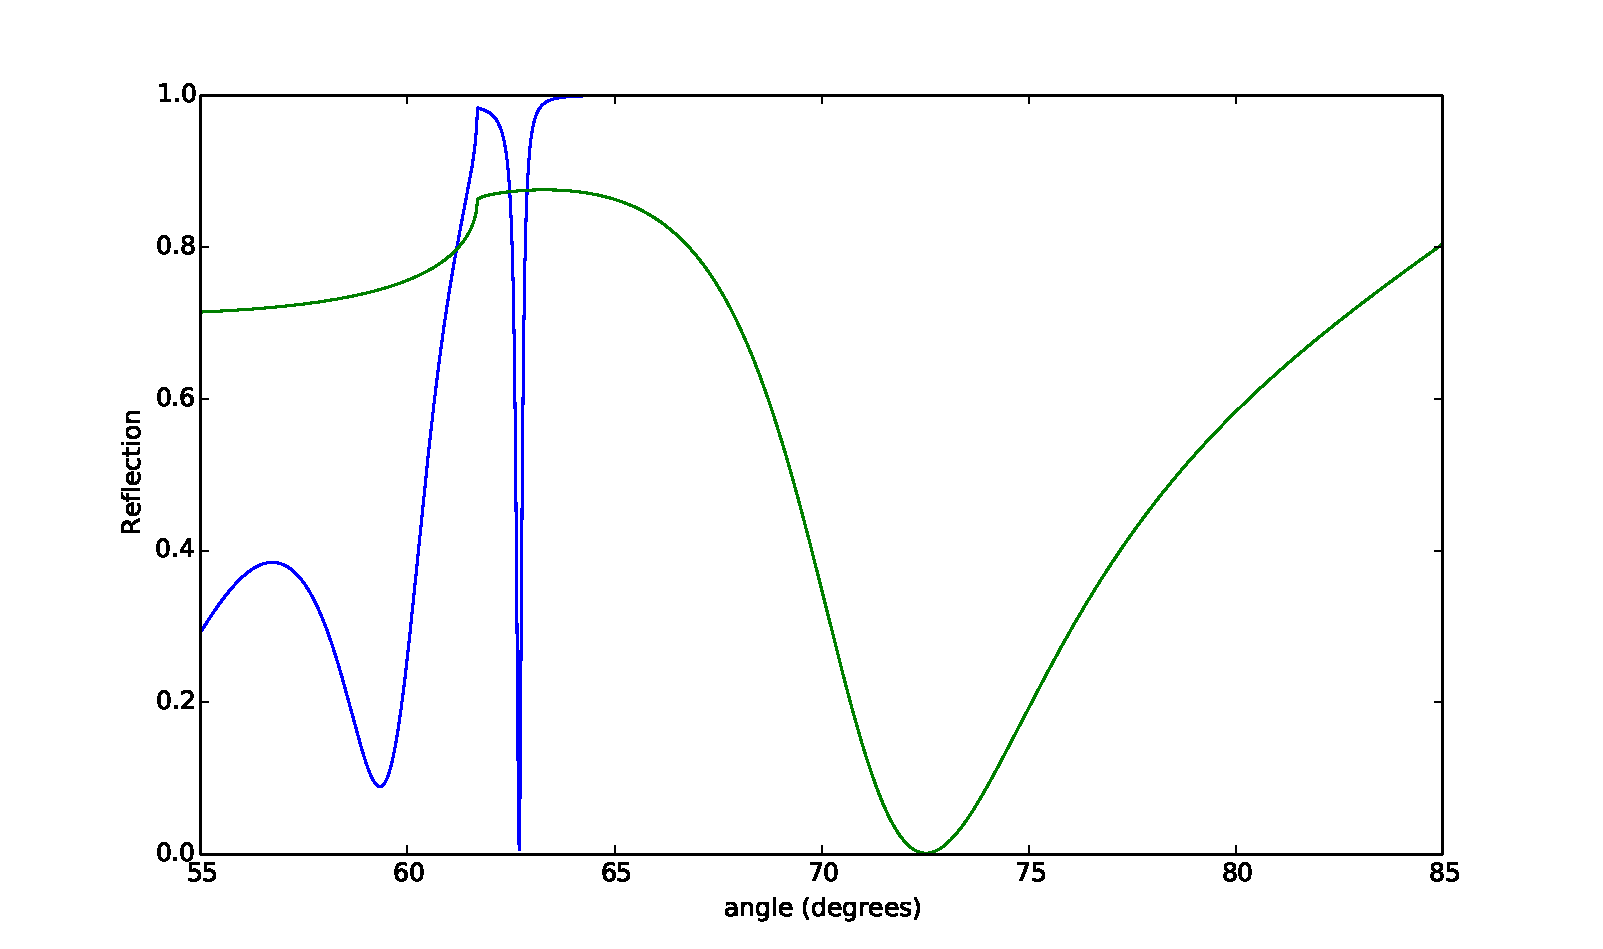
\includegraphics[width=0.9\textwidth,keepaspectratio]{figures/fresnelspp_ersatz.pdf}
%\caption{spp and lrspp, gold on cytop}
%% bk7 hemisphere 
%%x0 = array([ 1250e-9, 16e-9 ])
%%out = array([ fresnel(t,x0) for t in theta ])
%%x0 = array([ 1150e-9, 45e-9 ])
%% data in figures/data/spp_fresnel.dat
%\end{figure}
%
%\subsection{Physical Properties}
%Physical properties of SPP propagation are derived from $k_x$ and $k_z$.
%Since the SPP is confined to the plane of the metal, the surface plasmon
%wavelength $\lambda_\text{sp}$ is defined in terms of the real part of
%$k_x$
%\begin{align}
%\lambda_\text{sp} &= \frac{\lambda_0}{2 \pi} k_x\\
%& = \Re\left(\sqrt{
%  \frac {\epsilon_1+\epsilon_2}
%   {\epsilon_1 \epsilon_2 \lambda_0^2}
%}\right)
%\end{align}
%when $k_x$ is imaginary, \Equation{eqn:planewavexz} is evanescent in
%$x$ and the SPP decays with a characteristic $1/\me$ lifetime
%$\Im(1/(2k_x)$.  Similarly, when $k_{z,i}$ is imaginary, the
%$1/\me$ evanescent decay into either the metal or vacuum is given by
%$\Im(1/k_{z,i})$.  A table of these properties for many different SPP
%excitation configurations is found in \Appendix{ref:physicalproperties}.
%
%\section{Long Range Surface Plasmon Polaritons}
%The typical propagation distances for SPPs in the three layer Kretschmann
%configuration are on the order of $\SI{30}{\nano\meter}$ for Ag films and
%$\SI{6}{\nano\meter}$ for Au films.  The reason for this is the electric
%field extends into the metal and the real part of the metal's dielectric
%function damps the SPP oscillation, causing it to decay as heat.  However,
%if we are able to expel the SPP evanescent field from the metal region, the
%propagation distances can be extended orders of magnitude.  These are
%called \textit{long range surface plasmon polaritons} (LRSPPs), and in
%terms of our geometry can be excited in one of two ways.
%
%symmetric vs asymmetric spps
%
%\subsection{Symmetric Configuration}
%Cytop coating crap
%\subsection{Photonic Crystal Configuration}
%
%\section{Typical Response}
%some pictures of spp prop
%
%\chapter{Interference}
%
%\chapter{Experimental Setup}
%\label{ch:expsetup}
%
%The experimental setup is depicted schematically in
%\Figure{fig:sppexperimentalsetup}.  Light from a \SI{660}{\nano\meter}
%diode laser is first coupled into a single mode optical fiber.  The fiber
%guides the laser light to an optical breadboard mounted on an inverted
%microscope.  All primary functions of the experiment take place here.  The
%Gaussian output from the single mode fiber is collimnated with a beam waist
%$w_0=\SI{5}{\milli\meter}$ and proceeds
%through a polarizing beamsplitter, passing $p$ polarized light.  This light
%is focussed by a 10x microscope objective onto the
%hypotenuse of a hemispherical prism.  The prism is mounted on a planar
%structure supporting either normal or long range SPPs.  Reverse of this
%structure is a microfluidic flow cell where samples can be injected.  The
%specularly reflected and scattered light containing information from SPP
%interference and scattering is ultimately captured at desired locations by
%a pair of custom beam profilers. (notch filter).
%\begin{figure}
% \caption{Setup.}
% \label{fig:sppexperimentalsetup}
%\end{figure}
%
%\section{Planar Layer Structure}
%Perhaps most important to the setup is the layer structure supporting SPP
%propagation.  Two types of structures were created for this work: ones for
%SPPs and LRSPPs.
%
%
%\section{Spin Coater}
%During our experimental work, we did not have convienent access to a
%standard programmable spin coater.  This is of course a pre-requisite to
%producing uniform cytop coatings and thus long range surface plasmons.
%Being a rather expensive piece of equipment, we opted to build one
%ourselves using the brushless DC motor from a repurposed hard disk drive.
%Spin coaters built this way have been reported
%before~\cite{bianchi2006spin}, but we have made enough improvements on the
%design to justify its inclusion here.  Most significantly, the entire
%electronic drive and control are put together from off the shelf
%components.
%
%A block diagram of our home-built spin coater is shown in \Figure{fig:x}.
%The cover from a hard disk drive is removed and all of the internal
%components except for the motor are removed.  A solid aluminum plate is
%affixed to the top of the motor using the existing screw taps.  The motor
%is then connected directly to a programmable electronic speed controller
%(ESC).  The ESC itself is a standard component found in most land and air
%based radio controlled drones.  Once configured, the ESC accepts a pulse
%width modulated (PWM) input with pulse widths varying from \num{1000} (off)
%to \SI{2000}{\micro\second} (full speed).  The PWM signal for the ESC is
%generated by an Arduino Uno platform, based on the Atmel ATMega128
%\SI{8}{bit} microcontroller.  The Arduino can be programmed to do spins on
%its own, but we found it more convienent to send the desired spin speeds in
%real time to the Arduino via its USB serial interface.  Finally, connected
%to the motor spindle is a small flange and an optical interrupter switch
%which serves to monitor the spin speed.  
%
%We have experimented with using the optical interrupter as feedback for a
%proportional-integral-derivative (PID) loop in hopes that this would be a
%superior way of controlling the motor, but this idea was abandoned in favor
%of a proportional-only feedback loop.  The spin speed of the motor was also
%calibrated offline and a linear relationship with the PWM output determined
%such that it could function equally well without feedback.  
%
%The stability of the spin coater and the range of speeds it offers is shown
%in \Table{tbl:spincoatererror}.  Perhaps the most obvious downside of the
%ESC is that it does not operate very well in the low RPM limit.
%Fortunately, this is not an issue for us.
%
%brake on
%timing  high
%low voltage
%
%\begin{table}
% \begin{tabular}{ll}
%  \toprule
%  angular speed (RPM) & error \\
%  \midrule
%  1000 & x \\
%  2000 & x \\
%  3000 & x \\
%  4000 & x \\
%  5000 & x \\
%  6000 & x \\
%  7000 & x \\
%  \bottomrule
% \end{tabular}
% \label{tbl:spincoatererror}
%\end{table}
%
%\subsubsection{Determination of Film Thickness}
%\begin{equation}
% R = \frac{n_1^2(n_i-n_s)^2 \cos^2\delta + (n_i n_s - n_1^2)^2\sin^2\delta}
%          {n_1^2(n_i+n_s)^2 \cos^2\delta + (n_i n_s + n_1^2)^2\sin^2\delta}
%\end{equation}
%where
%\begin{equation}
%\delta = 2\pi/\lambda n_j d_j cos \theta
%\end{equation}
%
%\section{Cytop}
%poly(1,1,2,4,4,5,5,6,7,7-decafluoro-3-oxa-1,6-heptadiene) (Cytop).
%
%Cytop was purchased from AGC Chemicals as item number CTX-809A.  The last
%letter ``A'' in the item number designates it is intended for use on
%``amorphous'' (i.e. glass) applications, and the number immediately
%following that designates the concentration.  For example, CTX-809A is
%\SI{9}{\percent} cytop and \SI{91}{\percent} solvent, and likewise CTX-803A
%is \SI{3}{\percent} cytop and \SI{97}{\percent} solvent.
%
%refractive index reference: \cite{mikevs2005synthesis}
%
%
%
%\section{Chemistry and Surface Functionalization}
%esplandiu2002xps
%
%\section{Microfluidic Cell}
%
%\chapter{Interference}
%\label{ch:interference}
%Don't say this, but maybe say something like it
%Surface plasmon resonance is in of itself an interference phenomena: the dark band in the specular direction is due to interference between
%specularly reflected light and the re-radiated SPP which is likewise
%antiphase at the SPR resonance angle.  There is, however, a more rich 
%interference structure which can observed when using a focused beam whose spot size is smaller than the SPP propagation distance.  
%
%\section{Interference in Surface Plasmon Resonance}
%Perhaps the most 
%
%\section{The Fourier Optics Perspective}
%There are several perspectives of SPR phenomena which can be insightful in
%explaining why exactly the spatial oscillations are one-sided.  The first
%is an argument from causality.  Assume a complex function $\chi(\omega) =
%\chi'(\omega) + \mi \chi''(\omega)$ whose real and imaginary parts are
%related by Kramers-Kronig relations
%\begin{align}
%\chi(\omega)=\mi \hf{\chi(\omega)}
%\end{align}
%with 
%\begin{align}
%\chi'(\omega) &= \hf{\chi''(\omega)}\\
%\chi''(\omega) &= -\hf{\chi'(\omega)}
%\end{align}
%where $\hf{\chi(\omega)}$ is the Hilbert transform of $\chi(\omega)$.
%The Fourier transform of $\chi(\omega)$ is
%\begin{align}
%\chi(\omega) &= \chi'(\omega) + \mi \chi''(\omega)\\
%\ff{\chi(\omega)} &= \ff{\chi'(\omega) + \mi \chi''(\omega)}\\
%&= \ff{\chi'(\omega)} + \ff{\mi \chi''(\omega)}\\
%&= \ff{\chi'(\omega)} + \ff{\mi \hf{\chi'(\omega)}} \\
%&= \ff{\chi'(\omega)} + \sgn(\omega) \ff{\chi'(\omega)} \\
%\end{align}
%Or succinctly,
%\begin{align}
%\ff{\hf{\chi(\omega)}} = (-\mi \sgn(\omega)) \ff{\chi(\omega)}
%\end{align}
%In other words, the Fourier transform of any function which satisfies
%Kramers-Kronig relations is ``one-sided'' as a necessary
%condition of causality.  This seems to be true for the Fresnel
%reflectivity as well as the complex permittivity.
%
%The second perspective is couched in Fourier optics.  Here, because
%SPR occurs at the focus of a Gaussian beam, it can be seen as a sort of
%spatial filter which modifies the local $k$-vectors to produce
%the resulting far field optical pattern.  If the SPR resonance condition is
%sharp, the Fourier integral (\Equation{eqn:fourier123}) is truncated and
%the discontinuity acts as a low pass filter for light.  The one-sided
%oscillations are then essentially a manifestation of Gibb's phenomena.
%This seems to be well supported, because if the SPR resonance is broadened,
%say in the case of a BK7-Au-\ce{H2O} system, the interference is greatly
%attenuated.
%%
%%Another possible interpretation is that the near and
%%far field patterns in conically scattered light are qualatatively identical
%%to the simple impulse-response of a forced, damped harmonic oscillator.
%%This is of course equivalent to what the Lorentz-Drude model says about the
%%material properties.  The far field conically scattered light likewise
%%appears to be equivalent to the energy absorbed in the metal film which can
%%be detected as heat.
%
%\subsection{Specularly Directed Light}
%
%
%\subsection{Spatial Evolution}
%The Fresnel reflectivity predicts the far field angular distribution when
%illuminated by light at a specific angle, consisting of a single
%$k$-vector.  Now we will look at the evolution of light from this system
%as it propagates to the far field when excited by an incident Gaussian beam
%$g(x)$ containing a continuum of $k$-vectors.  We begin with treatment of
%light in the specular direction.  In the context of Fourier
%optics, the field on the surface in $k$-space is described by the Fourier
%decomposed incident Gaussian beam $\tilde{g}(k_x)$ multiplied by the
%Fresnel reflectivity
%\begin{align}
%\tilde{E}_\text{spec}(k_x)=\tilde{g}(k_x)\,\tilde{r}_\text{123}(k_x)
%\end{align}
%where
%\begin{align}
%\tilde{g}(k_x) = \intinfty g(x)\, \me^{\mi k_x x} \md x
%\end{align}
%and $g(x)$ represents a Gaussian beam in spatial dimensions.  We omit any 
%specific definition for $g(x)$ because its exact form
%is not important to our analysis.
%
%The complete optical field in both $x$ and $z$ can be obtained by computing
%the Fourier transform of $\tilde{E}_\text{spec}(k_x)$ multiplied 
%by the free space transfer function $\me^{\mi k_{z,1} z}$
%\begin{align}
%E_\text{spec}(x,z) &= \intinfty \tilde{E}_\text{spec}\, \me^{\mi k_{z,1} z}\, \me^{\mi k_x x} \md k_x\\
% &= \intinfty \tilde{g}(k_x)\, \tilde{r}_{123}(k_x)\, \me^{\mi \sqrt{k_0^2 \epsilon_1 - k_x^2}z}\, \me^{\mi k_x x} \md k_x
%\label{eqn:fourier123}
%\end{align}
%Likewise, conically scattered light may be found using the same treatment
%\begin{align}
%E_\text{cone}(x,z) = \intinfty \tilde{g}(k_x)\, \tilde{r}_{321}(k_x)\,\me^{\mi k_{z,1} z}\, \me^{\mi k_x x} \md k_x
%\label{eqn:fourier321}
%\end{align}
%Though this integral seems to have no analytic solution, its evaluation is
%nonetheless straightforward on a computer.
%The evolution of scattered and specularly directed light based on
%\Equation{eqn:fourier123} and \Equation{eqn:fourier321} is shown in
%\Figure{fig:fresnelpropagate} as a function of distance from the 2-3
%interface.  As can be seen, as the field propagates it diffracts,
%displaying a one-sided oscillatory structure. 
%
%\subsubsection{Evanescent Solutions}
%In the context of diffraction integrals, the free space transfer function
%$\exp(\mi k_{z,1} z)$ is often concerned with evanescent and propagating
%terms, giving rise to the diffraction limit.  Here,
%$k_{z,1}=\sqrt{k_0^2 \epsilon_1 - k_x^2}$ is imaginary for $k_0^2
%\epsilon_1 < k_x^2$.  It is interesting to note that this never occurs.
%Ignoring the condition for total internal reflection, 
%$k_x = k_0 \sqrt{\epsilon_1} \sin \theta$ and we can set up an inequality
%\begin{align}
%k_0^2 \epsilon_1 &< k_x^2\\
%k_0^2 \epsilon_1 &< \left(k_0 \sqrt{\epsilon_1} \sin \theta\right)^2\\
%k_0^2 \epsilon_1 &< k_0^2 \epsilon_1 \sin^2 \theta\\
%1 &< \sin^2 \theta
%\end{align}
%which is false, suggesting that if all light is collected, no information is
%lost during propagation from the near to far field.
%
%
%\chapter{Bulk Sensitivity}
%\label{ch:bulksensitivity}
%The sensitivity of surface plasmon based biosensors to bulk refractive
%index changes is of primary importance in extracting bio-relevant
%properties. In a prism coupled setup, there are three main modulation
%methods used to monitor changes in the SPR resonance.
%
%\begin{description}
% \item [{Angular}] The prism is rotated and the signal reflectivity
%  monitored
%  as a function of angle. The prism may be scanned through a range of
%  angles or the angular spectrum may be obtained simultaneously using
%  a focussed beam and sensor array.
% \item [{Wavelength}] The prism is fixed in place and its reflectivity at
%  a single angle is monitored as a function of wavelength.
% \item [{Intensity}] The intensity of the signal at a certain angular or
%  spatial point is monitored as the experiment progresses.
%\end{description}
%All three of these interrogation methods are equivalent in terms of
%their real-world resolution and detection limit. In this section we
%will look at the sensitivity of intensity interrogation to different
%(something about parameters)
%
%
%\section{Three Layer Kretschmann, Far Field}
%We will now derive the sensitivity of the three layer Kretschmann
%configuration to bulk index changes. This case will be used as a test
%case for further analysis of the propagation dependent sensitivity.
%
%The bulk sensitivity in an intensity modulation setup is defined as
%the ratio of the change of normalized signal intensity $\delta I=I_{n_{0}}-I_{n_{1}}$
%to the change in bulk refractive index $\delta n=n_{0}-n_{1}$ for
%two refractive indicies $n_{0}$ and $n_{1}$. We restrict ourselves
%to small changes in the refractive index $n$, $\delta n/n_{0}\ll1$.
%The intensity sensitivity is defined as
%\begin{equation}
%S_{\mathrm{I}}=\frac{\delta I}{\delta n}
%\end{equation}
%Without loss of generality, the sensor intensity $I$ may be a function
%of any appropriate coordinate system (e.g. $I(x,y)$). In such a coordinate
%system we always take $S_{\mathrm{I}}$ at the location of maximum
%shift in that coordinate system.
%
%In the Lorentzian approximation{[}{]} using Drude model coefficents
%$\epsilon=\epsilon'+\mi\epsilon''$, the maximum sensitivity for bulk
%index sensing is approximated as
%\begin{equation}
%(S_{\text{I}})_{\text{max}}=\frac{4\sqrt{3}}{9}\frac{\epsilon_{\mathrm{m}}'}{\epsilon_{\mathrm{m}}''n^{3}}
%\end{equation}
%Where $\epsilon_{\mathrm{m}}$ is the complex Drude-model permittivity
%in the metal layer. At a operating wavelength of \SI{660}{\nano\meter},
%for Au on N-BK7, $(S_{\mathrm{I}})_{\text{max}}=151.66$. This is
%only an approximation, though it is close to the value obtained through
%Lorentz-Drude coefficents used in combination with the transfer matrix
%method, $(S_{\mathrm{I}})_{\text{max}}=153.04$.
%
%\section{Long Range Surface Plasmons (Four Layer Kretschmann)}
%
%
%\subsection{Optimizing Sensitivity}
%
%The quoted values of $(S_{\mathrm{I}})_{\text{max}}$ depend on the
%refractive indicies of the system layers as well as the thickness
%of the metal layer. It is interesting to note that the maximum sensitivity
%does not coincide with maximum coupling of light into SPPs. The plot
%in Figure X shows the relationship between sensitivity and metal thickness.
%
%It can also be shown that the width of the signal is related to the
%sensitivity. 
%
%
%\section{Propagation Dependent Sensitivity}
%
%Having analyzed the classical case of SPR sensitivity in the three
%layer Kretschmann configuration, we are now ready to look at the propagation
%dependent sensitivity. 
%
%
%\subsection{Theoretical Maximum Sensitivity for an Arbitrary Signal}
%
%Consider an arbitrary complex signal of some coordinate $f(x)$ such
%that the indefinite integral
%\begin{equation}
%\int_{-\infty}^{\infty}|f(x)|^{2}\md x=\text{(some finite value)}
%\end{equation}
% and
%\begin{equation}
%\lim_{x\to\pm\infty}|f(x)|^{2}=0
%\end{equation}
%Specifically $f(x)$ must be \textit{band-limited}. Following, it is
%completely determined by its Fourier series.
%
%1/range is the spacing
%1/dx is the range
%minimum frequency is zero (nyquist)
%maximum frequency is N/range
%
%maximum frequency determines the maximum derivative of the signal
%
%% We have to choose a resolution for sampling so that we introduce no error
%% in the signal.  So the band in which we cut off is determined by the
%% error we're willing to deal with.
%
%% Just define error as the least squares error
%% choose bounds such that the least squares error is at most x
%% 
%
%
%
%\section{Conically Scattered Light}
%
%As described in X, light can also be directionally scattered into
%the cone. This propagation contains the same interference structure
%as the specularly reflected light, and is likewise subject to the
%same analysis.
%
%
%\section{Multiple Scattering Effects}
%
%It is known that a speckle field with multiple scattering effects
%is more sensitive to some kind of fixed phase stuff 
%
%\chapter{Speckle}
%\label{ch:speckle}
%
%Light can be scattered into the cone, see the original paper by Kretschmann
%and the one that's paired with it... Matthew gave you both of them.
%
%\section{Statistical Properties of the Cone Speckle}
%% Ideas for this section: take some pictures of the cone speckle and run it
%% through the treatment provided by goodman.  Make some inferences on
%% whether it's gaussian or not or whatever.
%
%\section{Non-Paraxial Speckle}
%
%
%\section{Optical Vorticies}
%% vortex tracking stuff
%
%
%\chapter{Simulations}
%\label{ch:simulations}
%A parallel Monte Carlo simulation was written to model surface plasmon
%random scattering in our experiment. This simulation is capable of modeling
%a comprehensive set of phenomena expected to exist in this work: single
%scattering, multiple scattering, the effects of moving scatterers, and the
%effects of adding scatterers. The simulation assumes a geometery shown in
%Figure X, consisting of:
%
%\begin{itemize}
%
%\item A \textit{scatterer}, a fixed point where an SPP can scatter to
%another scatterer or exit the system to the far field.
%
%\item An elliptical \textit{illuminated region}, representing the incident
%evanescent field which excites SPPs.
%
%\item A \textit{trajectory} or \textit{path}, meaning the ordered sequence
%of scatterers a plasmon visits before exiting the system. This path is
%characterized by its path length and mean free path. A path always begins
%in the illuminated region.
%
%\end{itemize}
%
%The plasmon is assumed to propagate according to the time independent
%monochromatic wave equation, $\mathbf{E}(\mathbf{r})=\me^{\mi
%\mathrm{k}\cdot \mathrm{r}}$, where $\mathrm{k}$ is the plasmon wavevector
%and $\mathrm{r}$ is the spatial variable.
%
%\section{Single Scattering}
%
%\section{Multiple Scattering}
%
%\chapter{Multiple Scattering of SPPs}
%\section{Speckle}
%\section{Optical Vorticies}
%% pseudophase algorithm
%
%\chapter{The Moving Scatterer Problem}
%\section{Weirdospace}
%\section{Reverse Mapping}
%
%%\import{wiggles/}{fig2}
%
%%\begin{figure}
%%\centering
%%
\includegraphics{tmp/out.pdf}
%%\caption{How do the font sizes look?}
%%\end{figure}
%
%
%\section{Colophon}
%This document was typeset using pdf\TeX. All plots were rendered using
%pgfplots~\cite{feuersangerpgfplots} with styles influenced by
%\name{Eduard~Tufte}~\cite{tufte1983visual}~\cite{tufte1991envisioning}.
%Colors were chosen from datasets provided by
%\name{Jan~Brewer}~\cite{harrower2003colorbrewer}.  Schematics and other
%line drawings were prepared using Inkscape. Generation of text was done
%under Arch Linux using \texttt{vim}.  Some tables were pre-processed using
%LyX.
%
%The Monte Carlo simulations were written in \texttt{c} with parallelism
%accomplished using \texttt{mpi}. The vortex tracking and image processing
%algorithms were written in \texttt{octave}.  Weirdospace images were
%processed using python and scipy/numpy.  Parallel execution when required
%was done at at the FAU RRZE, Erlangen, Germany.  Multiple scattering code
%written by \name{Matthew~Foreman} was written in \texttt{MATLAB}.  All sources
%available through the author.
%
%\chapter{Reference Data}
%Several datasets were produced during the course of this dissertation which
%might be useful to the reader.  They are presented here.
%\section{Physical Properties of SPP Propagation}
%\label{ref:physicalproperties}
%%\import{dispersion/}{sptable_632.tex}
%\section{The Three Layer Fresnel System}
%%% you will have to fix the path in the following file
%%\import{fresnel_plots/}{allthreelayerfresnel}
%
%\section{Complex Permittivities and Permiabilities of Metals}
%%\import{eps_plots/}{allmetals}
%
%
%\section{Abbreviations}
%%\begin{table}
%% \begin{tabular}
%%  SPP & surface plasmon polariton
%%  LRSPP & long range surface plasmon polariton
%% \end{tabular}
%%\end{table}
%
%for plasma bonding I do exactly this:
%http://umech.mit.edu/HST410/plasma.php

% layer fitting
\bibliographystyle{plain}
\bibliography{bibliography}

\end{document}

% MISSING A HOME
% surface roughness parameters
